\documentclass{article}
\usepackage{amssymb}
\usepackage{amsmath}
\usepackage{hyperref}
\usepackage{tikz}
\usepackage[a4paper]{geometry}
\usepackage{fancyhdr}
\pagestyle{fancy}
\lhead{Das Doppelspaltexperiment}
\rhead{September 2025}
\begin{document}
\section{Das Doppelspaltexperiment} 
Wird ein Lichstrahl eines Lasers (oder der Lichtstrahl einer Lampe, welche durch mehrere Linsen und Gitter gegangen ist) durch einen \emph{Doppelspalt} geschien, so ensteht auf den hinterliegenden Schirm ein \emph{Interferenzmuster}. 
 
\noindent \begin{minipage}{\dimexpr\linewidth-8cm}
 Dem \hyperref[Ausbreitung]{Huygenschen Prinzip} nach breitet sich das Licht von A und B aus als Elementarwellen in Richtung des Schirms aus. Kommt das Licht beide Spalte bei P mit einem Gangunterschied $\Delta = \text{BK}$ als ein Vielfaches der Wellenlänge an, also $\Delta = k \cdot \lambda$ mit $k \in \mathbb{N}$, so liegt ein Maximum vor.
\end{minipage} 
\hfill 
\begin{minipage}{7.5cm}
 \center
 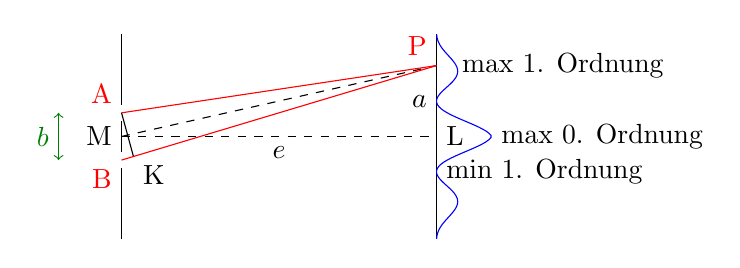
\begin{tikzpicture}
  \draw (0, -0.2) -- (0, 0.2);
  \draw (0, 0.4) -- (0, 1.3);
  \draw (0, -0.4) -- (0, -1.3); 
 
  \draw (4, -1.3) -- (4, 1.3); 
  \draw[domain=-1.3:1.3,variable=\y,blue,samples=100]
    plot ({4+0.5*(1+cos(7*\y r))*(0.7-abs(0.5*\y))},\y);
 
  \draw[dashed] (0, 0) -- (4, 0) node [pos=0, left] {M} node [pos=0.5, below] {$e$} node [pos=1, right] {L}; 
  \draw[dashed] (0, 0) -- (4, 0.9);
  \draw[red] (0, 0.3) -- (4, 0.9) node [pos=0, above left] {A} node [pos=1, above left] {P};
  \draw[red] (0, -0.3) -- (4, 0.9) node [pos=0, below left] {B};
  \draw (0, 0.3) -- (0.15, -0.25) node [below right] {K};
  \draw (4, 0.44) node [left] {$a$};
  
  \draw (4.2, 0.9) node[right] {max 1. Ordnung};
  \draw (4.7, 0) node[right] {max 0. Ordnung};
  \draw (4, -0.448) node[right] {min 1. Ordnung};
 
  \draw[green!50!black, <->] (-0.8, -0.3) -- (-0.8, 0.3) node [midway, left] {$b$};
 
 \end{tikzpicture} 
\end{minipage} 
\subsection{Maximumsbedingung}
Es liegt ein Maximum vor, wenn
\[
 \Delta = k \cdot \lambda
 \quad \text{mit} \quad
 k \in \mathbb{N}
\] 
Wird angemerkt, dass in der Abbildung in $\Delta \text{ABK}$ immer $\sin\alpha = \dfrac{\Delta}{b}$ und in $\Delta \text{MLP}$ dann ${\tan\alpha = \dfrac{a}{e}}$ gilt, so folgt
\[
 \Delta = \lambda \cdot k = b \cdot \sin{\left(\arctan{\left(\frac{a}{e}\right)}\right)} 
\]
\subsection{Minimumsbedingung}
Ein Minimum tritt auf, wenn sich die beiden Strahlen maximal auslöschen, wenn eine maximale Interferenz vorliegt. Dies ist der Fall, wenn es einen Phasenunterschied von $1/2 \,\lambda$ gibt, also wenn
\[
 \Delta = \frac{1}{2} \left(2k+1\right) \lambda
 \quad \text{mit} \quad
 k \in \mathbb{N}
\] 
\end{document}